% ============================================================================================
% astar_fap.tex -- the two non-HTN formulations in the repository: flat-state A* search
% (spider_web_astar/) and the fixed-action-pattern model (spider_web_fap/, run_fap.py).
% Fragment (no preamble). Figures under figures/astar_fap/, generated by scripts/astar_fap/*.
% Repository state: commit 61d18d8. All planner runs are ours, made in private copies of the
% repository at 61d18d8 and at 1e1bd44 (see the MANIFEST); raw records in
% work/astar_fap/data/runs.jsonl and witness_*.json.
% Extra bibliography entry: sections/astar_fap.bib (ghallab2016automated).
% ============================================================================================
\providecommand{\code}[1]{\texttt{#1}}

\section{Alternative Formulations: A* Search and a Fixed-Action-Pattern Model}
\label{sec:astar_fap}

The repository contains two formulations of orb-web construction that are not HTN models in the
sense of the Checkpoint~2 report, and which that report does not mention. The
\emph{fixed-action-pattern} (FAP) model (\code{spider\_web\_fap/\allowbreak{}}, entry point \code{run\_fap.py})
was part of the very first commit (\code{d0a472a}, 2026-08-04, ``first 2 implementations'')
alongside the original HTN package. A \emph{flat-state A*} planner (\code{spider\_web\_astar/\allowbreak{}})
was added on 2026-08-30 (\code{1e1bd44}), together with an ethological data table
(\code{spider\_web\_astar/\allowbreak{}empirical\_data.md}) and an exported plan; the plan and a copy of the plan
viewer (\code{visualization/\allowbreak{}index\_astar.html}, \code{plan\_data\_astar.js}) were moved into
\code{visualization/\allowbreak{}} on 2026-09-04 (\code{b6793d0}). Neither package is used by the comparison
and sensitivity scripts of the updated HTN package, which use the random-walker baseline instead.
The repository's own notes call the A* module ``a superseded early attempt'' that ``fails to find a
plan within its own default budget'' (\code{insights.md}, 2026-09-09), and the research README
states that the FAP and A* packages ``have not all been independently audited''. This section is
that audit. It states both formulations precisely, re-runs them, and sets them beside the two HTN
models on the same rig. In line with claim C17 of the repository's claim ledger
(\code{docs/\allowbreak{}research/\allowbreak{}CLAIMS.md}: the packages do \emph{not} yet support one joint quantitative
conclusion), the comparison in Section~\ref{sec:astar_fap-compare} describes the planners side by
side. It does not rank them.

% --------------------------------------------------------------------------------------------
\subsection{The A* formulation}
\label{sec:astar_fap-astar}

\paragraph{State.}
A* reuses the state object and primitive operators of the original HTN package
(\code{spider\_web\_htn/\allowbreak{}state.py}, \code{operators.py}) on the same Zschokke rig (two 18\,cm sticks
16\,cm apart, one crossbar, 17 named structure and anchor nodes) with the spider released at
\code{right\_stick\_top}. For duplicate detection, \code{state\_key} maps a state to the hashable
tuple
\begin{equation}
  \kappa(s) = \bigl(p,\ \mathrm{set}(E),\ N,\ \eta,\ \eta_{\mathrm{pos}},\ n_{\mathrm{pr}},\ n_{\mathrm{r}},\
  n_{\mathrm{f}},\ \beta_{\mathrm{top}},\ \beta_{\mathrm{hub}},\ \beta_{\mathrm{aux}},\
  \beta_{\mathrm{cap}},\ \beta_{\mathrm{web}},\ \beta_{\mathrm{bridge}},\ \beta_{\mathrm{high}}\bigr),
  \label{eq:astar_fap-key}
\end{equation}
where $p$ is the spider's position, $E$ the list of typed threads $(u,v,\tau)$ (hashed as a set, so
two identical threads collapse in the key but not in the counters), $N$ the known nodes, $\eta$ and
$\eta_{\mathrm{pos}}$ the proto-hub flag and position, $n_{\mathrm{pr}}, n_{\mathrm{r}}, n_{\mathrm{f}}$
the proto-radius, radius and frame counters and the $\beta$ the remaining progress flags. Energy is
not part of the key; it is the path cost $g$.

\paragraph{Operators and costs.}
A* has no method library. Each generator in \code{spider\_web\_astar/\allowbreak{}operators.py} enumerates
ground instances of one HTN primitive, applies it to a copy of the state and yields
$(a, c(a), s')$, with $c(a)$ the increase of \code{energy\_expended}. This is the Euclidean
length of the move or thread in centimetres (the locomotory-energy proxy of Section~5 of the
Checkpoint~2 report), and zero for bookkeeping actions (Table~\ref{tab:astar_fap-ops}). The
generators add restrictions that the HTN methods otherwise supply (distance caps, ``hub before
frame before spiral'' gates). The \code{anchor} generator exists but is not called
(``fixed-geometry experiment''). At the initial state 32 successors are generated (walk~5,
lay\_thread~14, drop\_down~8, swing\_tarzan~4, attach\_dragline~1). Over the successful search
reported below, 6,358 states are generated for 227 expanded, about 28 per expansion.

\begin{table}[htbp]
\centering
\small
\caption{A* successor generators (\code{spider\_web\_astar/\allowbreak{}operators.py}) and their costs.
$d(u,v)$ is the Euclidean distance between node coordinates in cm. ``Anchors'' are the eight
\code{anchor\_*} nodes; frame targets are those eight plus the two stick tops.}
\label{tab:astar_fap-ops}
\begin{tabularx}{\linewidth}{@{}l X l@{}}
\toprule
Generator & Ground instances offered in state $s$ & Cost \\
\midrule
\code{walk} & one hop along a structural edge or an existing thread & $d(p,v)$ \\
\code{lay\_thread} & dragline to any known node within 20\,cm with no thread to $p$ yet & $d(p,v)$ \\
\code{drop\_down} & dragline to any node 0--15\,cm lower (no horizontal limit) & $d(p,v)$ \\
\code{swing\_tarzan} & dragline to any node within 10\,cm (no duplicate check) & $d(p,v)$ \\
\code{attach\_dragline}, \code{remove\_thread} & no-op at $p$; delete a thread incident to $p$ & 0 \\
\code{reel\_up} & move along a thread incident to $p$ & $d(p,v)$ \\
\code{insert\_radius} & convert a dragline from $p$ to an anchor into a proto-radius & 0 \\
\code{mark\_proto\_hub} & at $p$, if $n_{\mathrm{pr}}\ge 3$ (the operator itself requires $\ge 4$) & 0 \\
\code{lay\_frame\_thread} & hub exists; to any frame target; sets $\beta_{\mathrm{top}}$ if the target is \code{anchor\_top\_center} & $d(p,v)$ \\
\code{lay\_radius} & spider at the hub; to any anchor (spider ends at the anchor) & $d(p,v)$ \\
\code{build\_spiral\_segment} & $\beta_{\mathrm{top}}$; to any reachable node with no thread to $p$; auxiliary type until four exist, then capture & $d(p,v)$ \\
\code{mark\_web\_complete} & $n_{\mathrm{f}}\ge 2$, $n_{\mathrm{r}}\ge 4$, capture spiral done & 0 \\
\bottomrule
\end{tabularx}
\end{table}

\paragraph{Goal test.}
With the thresholds of \code{spider\_web\_astar/\allowbreak{}state.py} (\code{GOAL\_THRESHOLDS}),
\begin{equation}
  G(s) \iff \beta_{\mathrm{web}} \wedge \eta \wedge n_{\mathrm{f}}\ge 2 \wedge n_{\mathrm{r}}\ge 4
  \wedge \#\{\tau=\text{capture}\}\ge 4 ,
  \label{eq:astar_fap-goal}
\end{equation}
and capture segments can only be laid after four auxiliary segments. The test is purely a count.
It does not ask for distinct anchors, an interior hub or any geometric property of the result,
and this decides what A* produces (Section~\ref{sec:astar_fap-web}). These targets are also far
smaller than what the HTN plans build (8~radii and 4~frame threads; Table~\ref{tab:astar_fap-compare}).

\paragraph{Heuristic: intended and actual.}
\code{heuristic.py} documents a ``Stage~4'' bound. Let $R, F, A, C$ be the remaining radii, frame
threads, auxiliary and capture segments, $t=[\neg\beta_{\mathrm{top}}]$, and let $\delta_X$ be the
smallest \emph{strictly positive} distance from a known node to a node of the set $X$. The
intended heuristic is
\begin{equation}
  h(s) = R\,\delta_{\mathrm{anchors}}
  + \begin{cases}
      \delta_{\mathrm{top}} + (\max(F,t)-1)\,\delta_{\mathrm{frame}} & t=1\\
      F\,\delta_{\mathrm{frame}} & t=0
    \end{cases}
  + (A + C)\,\delta_{\mathrm{any}} ,
  \label{eq:astar_fap-h}
\end{equation}
with $h=0$ once $\beta_{\mathrm{web}}$ holds; proto-radii are not counted. The code does not
compute Equation~\eqref{eq:astar_fap-h}. Its helpers pass coordinate \emph{tuples} to
\code{spider\_web\_htn.utils.calculate\_distance}, which expects node \emph{names}. In the version
committed with the A* package (\code{1e1bd44}), unknown names fell back to a fixed cost of
2.0\,cm, so every $\delta$ evaluated to 2 and
\begin{equation}
  h_{\mathtt{1e1bd44}}(s) = 2\,\bigl(R + \max(F,t) + A + C\bigr),\qquad h_{\mathtt{1e1bd44}}(s_0)=28 .
  \label{eq:astar_fap-h-old}
\end{equation}
On 2026-09-04 (\code{60be973}, ``Debugging'') \code{calculate\_distance} was changed to map any
unknown name to the default hub coordinate $(8,12)$. Both tuples now map to the same point, every
$\delta$ is 0, and at \code{61d18d8}
\begin{equation}
  h_{\mathtt{61d18d8}}(s) \equiv 0 .
  \label{eq:astar_fap-h-head}
\end{equation}
None of the A* files changed, but a change in the shared HTN utilities silently turned the
heuristic off. With $h\equiv 0$ the weight $w$ in $f=g+wh$ has no effect, and the search is
uniform-cost search with a tie-breaker. We also ran a one-line repair of our own (Euclidean
distance on the tuples, i.e.\ Equation~\eqref{eq:astar_fap-h} as documented; not repository
code), labelled ``h-fix'' below, with $h(s_0)=47$.

\paragraph{Admissibility and consistency.}
The docstring says admissibility was ``checked (not proven)'' by replaying one plan through
\code{validate\_heuristic.py}. That file is not in the repository. From the code, none of the three
variants is both informative and admissible. The intended bound assumes that every remaining
counted action costs at least the smallest \emph{positive} distance. However,
\code{bottom\_path} and \code{anchor\_bottom\_center} have the same coordinates $(8,0)$, so a
radius, frame thread or spiral segment between them costs exactly 0. We built the state $S$ by an
action sequence that we checked step by step against the generator (\code{astar\_witness.py}): the
hub is at \code{bottom\_path}, the frames and both spirals are complete, no radius is laid yet, and
the spider is at the hub. The remaining cost is $h^*(S)=0$: four zero-cost
\code{lay\_radius}/\code{walk} pairs, which A* from $S$ finds in 12 expansions. Yet
$h_{\mathtt{1e1bd44}}(S)=8$ and $h_{\text{h-fix}}(S)=12$, so both are inadmissible. They are also
inconsistent: on the zero-cost edge \code{lay\_radius(bottom\_path, anchor\_bottom\_center)} $h$
falls by 2 (or 3) while $c=0$, and five such violations occur along a single plan. Only
$h\equiv 0$ is admissible and consistent, and it carries no information. Since \code{find\_plan}
is in any case run with $w=3$ by default, the returned plans carry no optimality guarantee. They
are not optimal. A complete 33-action plan that uses the zero-length pair as the hub
(radii and one frame thread at zero cost, then the top frame and eight spiral segments) costs
71.70\,cm, compared with 75.54\,cm for the committed A* plan (witness files
\code{witness\_*.json}). For $h\equiv 0$ the minimum $f$ left in OPEN at a cutoff is a valid lower
bound, although \code{astar.py} labels it unsound whenever $w>1$. The 120\,s run below therefore
brackets the optimal cost of this goal between 19.70 and 71.70\,cm.

\paragraph{Search procedure and tie-breaking.}
Algorithm~\ref{alg:astar_fap-astar} states \code{astar.find\_plan}. It is textbook
A*~\cite{ghallab2016automated} with lazy deletion and a closed set. Heap entries are
$(f, -\pi, g, \text{counter}, \kappa, s)$, where $\pi(s)=-(\text{remaining mandatory actions})$ is
the progress score of \code{heuristic.py}. Among equal $f$, the planner prefers more completed work,
then lower $g$, then earlier generation. Generation order follows iteration over the Python sets
$N$ and $E$, so it depends on the interpreter's string-hash seed. Across ten runs with
\code{PYTHONHASHSEED}$=0,\dots,9$ the committed code returned six different 26-action plans:
eight cost 75.54\,cm and two (seeds 7 and 9) cost 85.54\,cm. The two committed plan files are
reproduced exactly, \code{visualization/\allowbreak{}plan\_data\_astar.js} by seed~4 and the older copy in
\code{spider\_web\_astar/\allowbreak{}visualization/\allowbreak{}} by seeds 1, 3, 6 and~8.

\begin{algorithm}[htbp]
\caption{Weighted A* as implemented in \code{spider\_web\_astar/\allowbreak{}astar.py}}
\label{alg:astar_fap-astar}
\begin{algorithmic}[1]
\Require initial state $s_0$, weight $w$, time budget $T$, expansion budget $M$
\State $\mathit{OPEN}\gets\{(g_0+w\,h(s_0),\,-\pi(s_0),\,g_0,\,0,\,\kappa(s_0),\,s_0)\}$;
       $\mathit{CLOSED}\gets\emptyset$; $\hat g[\kappa(s_0)]\gets g_0$
\While{$\mathit{OPEN}\neq\emptyset$}
  \If{elapsed $\ge T$ \textbf{or} expansions $\ge M$}
    \State \Return failure, the best-progress state, $\min f$ in $\mathit{OPEN}$
  \EndIf
  \State pop the lexicographically smallest $(f,-\pi,g,\cdot,\kappa,s)$
  \If{$g>\hat g[\kappa]$ \textbf{or} $\kappa\in\mathit{CLOSED}$} \textbf{continue} \Comment{stale entry}
  \EndIf
  \State $\mathit{CLOSED}\gets\mathit{CLOSED}\cup\{\kappa\}$
  \If{$G(s)$} \Return the plan by parent pointers \EndIf
  \ForAll{$(a,c,s')\in\textsc{Successors}(s)$} \Comment{Table~\ref{tab:astar_fap-ops}}
    \State $g'\gets g+c$
    \If{$\kappa(s')\notin\mathit{CLOSED}$ \textbf{and} $g'<\hat g[\kappa(s')]$}
      \State $\hat g[\kappa(s')]\gets g'$; parent$[\kappa(s')]\gets(\kappa,a)$
      \State push $(g'+w\,h(s'),\,-\pi(s'),\,g',\,\text{counter},\,\kappa(s'),\,s')$
    \EndIf
  \EndFor
\EndWhile
\State \Return failure
\end{algorithmic}
\end{algorithm}

% --------------------------------------------------------------------------------------------
\subsection{Measured search effort}
\label{sec:astar_fap-effort}

We ran \code{find\_plan} on the initial state in private copies of the repository at the A*
commit \code{1e1bd44} and at \code{61d18d8} (\code{run\_measurements.py}, one process per run,
\code{PYTHONHASHSEED}$=0$ unless stated). Table~\ref{tab:astar_fap-runs} and
Figures~\ref{fig:astar_fap-path} and~\ref{fig:astar_fap-scaling} give the results.

\begin{table}[htbp]
\centering
\small
\caption{A* runs on the default goal (Eq.~\ref{eq:astar_fap-goal}). ``Exp.''/``Gen.'' are states
expanded/generated, ``OPEN'' the largest heap size. Runs that hit the time budget report the
budget-limited counts. 1e1bd44 runs used a 120\,s budget, \code{61d18d8} default runs the repository
default (120\,s, 200,000 expansions), h-fix runs 60\,s. Source: \code{runs.jsonl}.}
\label{tab:astar_fap-runs}
\footnotesize
\setlength{\tabcolsep}{4pt}
\begin{tabular}{@{}llrrrrrr@{}}
\toprule
Code & $w$ & Plan & Cost (cm) & Exp. & Gen. & OPEN & Time (s) \\
\midrule
1e1bd44 & 3 & 26 & 75.54 & 227 & 6,358 & 6,132 & 0.58 \\
1e1bd44, seeds 0--9 & 3 & 26 & 75.54 / 85.54 & 226--231 & 6,340--6,544 & 6,115--6,314 & 0.56--0.59 \\
1e1bd44 & 1 & -- & -- & 35,198 & 1,012,585 & 977,345 & 120 \\
1e1bd44 & 1.5 & -- & -- & 35,313 & 1,015,815 & 980,460 & 120 \\
1e1bd44 & 2 & -- & -- & 31,646 & 892,513 & 860,863 & 120 \\
1e1bd44 & 5 & -- & -- & 30,940 & 881,380 & 850,440 & 120 \\
1e1bd44 & 10 & -- & -- & 31,569 & 899,316 & 867,747 & 120 \\
61d18d8 ($h\equiv0$) & 3 & -- & -- & 25,839 & 727,934 & 702,053 & 120 \\
61d18d8 + h-fix & 1 & -- & -- & 26,340 & -- & -- & 60 \\
61d18d8 + h-fix & 3 & -- & -- & 20,633 & -- & -- & 60 \\
61d18d8 + h-fix & 5 & -- & -- & 20,729 & -- & -- & 60 \\
\bottomrule
\end{tabular}
\end{table}

\paragraph{As committed (1e1bd44).}
With the repository's default weight $w=3$, A* returns a 26-action plan of 75.54\,cm after 227
expansions in 0.58\,s. Every other weight we tried fails within 120\,s, including the admissible
setting $w=1$ (which with this heuristic is not admissible anyway): $w=1, 1.5, 2, 5, 10$ all stop
after 30,940--35,313 expansions and 0.85--1.0 million generated states. Along the returned plan
(Fig.~\ref{fig:astar_fap-path}a), $h$ stays at 28 for the first ten states (proto-radii are not
counted) and then falls by 2 per counted action. It never exceeds the plan's remaining cost, the
only check the docstring reports, but that check cannot detect the violation shown above. The
heap trace (Fig.~\ref{fig:astar_fap-path}b) shows $f$ rising from 84 to 96 and then dropping to
the goal at 75.54, as expected when $w>1$. Varying the goal size $k$ (both the radius and the
capture-segment thresholds set to $k$; auxiliary segments fixed at 4) gives plans of 18 to 38
actions and 46.0 to 116.54\,cm. Expansions grow from 106 ($k=1$) to 1,199 ($k=8$), and generated
states from 2,181 to 39,515 (Fig.~\ref{fig:astar_fap-scaling}a). In this narrow configuration the
planner scales smoothly. We read that as the luck of one tie-breaking order, not robustness: the
weight sweep shows that a small change to the search makes it fail.

\paragraph{At the current commit (61d18d8).}
With $h\equiv 0$ the default call (\code{main.py}: $w=3$, 120\,s, 200,000 expansions) finds no
plan. It expands 25,839 states, generates 727,934 and holds up to 702,053 in OPEN. The deepest node is at depth 56, and the minimum $f$ in OPEN reaches only 19.70\,cm,
the cost of the single \code{lay\_thread} from \code{right\_stick\_top} to \code{bottom\_path}
(Fig.~\ref{fig:astar_fap-path}b). This reproduces the note in \code{insights.md} (``$\sim$25k
nodes expanded, no solution''). The cause is the heuristic defect described above, not the
intractability that the note gives. Uniform-cost search must exhaust a large plateau of zero- and
low-cost states (\code{insert\_radius}, \code{remove\_thread}, \code{attach\_dragline} and
zero-length moves at $(8,0)$) before $g$ can grow. Even the smallest goals ($k=1,2,3$) fail within
60\,s at 14,079--14,212 expansions. Our h-fix variant fails at every weight and every $k$
tried within 60\,s (20,190--26,448 expansions; Fig.~\ref{fig:astar_fap-scaling}). The
best-progress states of these runs typically have frames and spirals finished but radii still
missing. So the plan in the repository and its viewer can no longer be regenerated by
\code{visualize\_astar.py} at the current commit.

\begin{figure}[htbp]
\centering
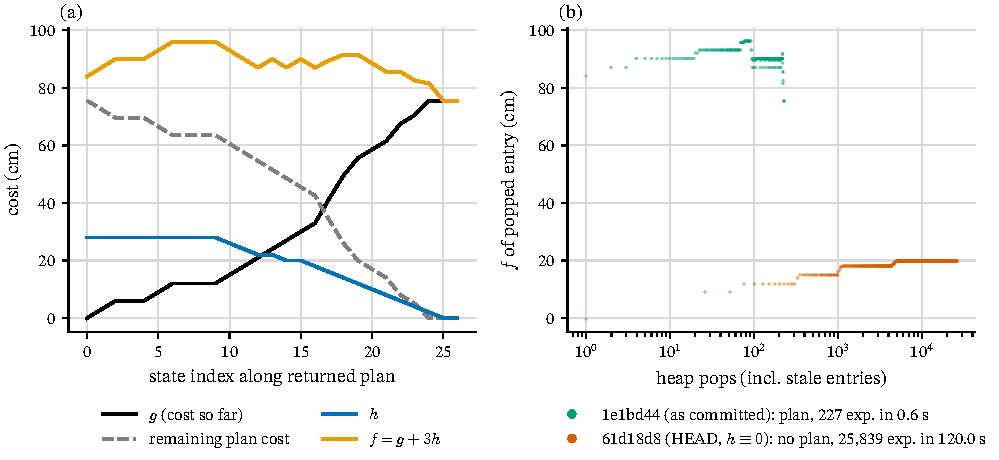
\includegraphics[width=\linewidth]{figures/astar_fap/astar_search_path}
\caption{A* search behaviour. (a) Cost so far $g$, heuristic $h$, priority $f=g+3h$ and the
remaining cost of the returned plan, at each state along the 26-action plan found by the A* code
as committed (\code{1e1bd44}, $w=3$). The plan is not optimal, so the dashed line is an upper bound
on the true cost-to-go. (b) $f$ of every popped heap entry (stale entries included) against pop
index, for that run (green, 227 expansions, every pop) and for the default run at the current
commit \code{61d18d8} where $h\equiv0$ (vermillion, every 25th pop shown, no plan within 120\,s).
$n=1$ run each; our runs, \code{runs.jsonl} tags \code{astar\_old\_trace} and
\code{astar\_head\_default}; code \code{spider\_web\_astar/\allowbreak{}astar.py}.}
\label{fig:astar_fap-path}
\end{figure}

\begin{figure}[htbp]
\centering
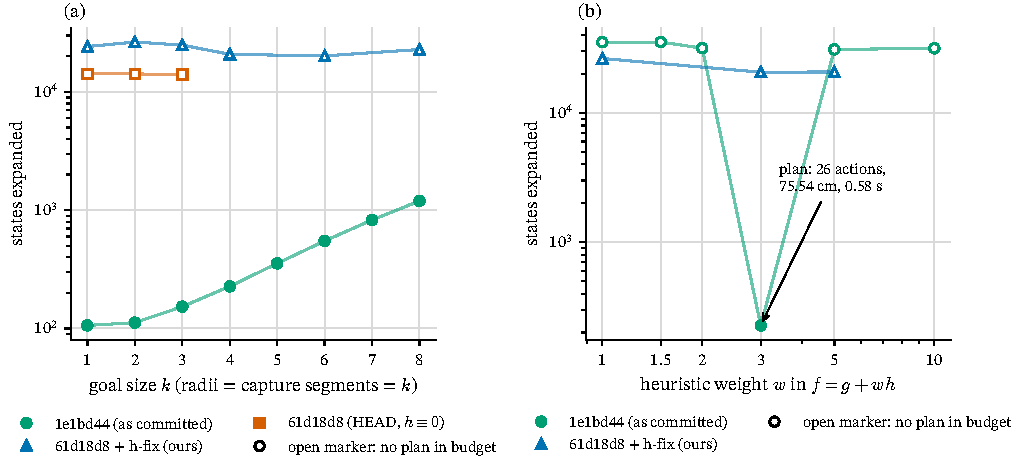
\includegraphics[width=\linewidth]{figures/astar_fap/astar_scaling}
\caption{How A* search effort depends on problem size and weight. (a) States expanded against goal
size $k$ (\code{min\_radii} $=$ \code{min\_capture\_spiral} $=k$, $w=3$). (b) States expanded against
the weight $w$ (default goal $k=4$). Filled markers: plan found. Open markers: no plan within the
budget, plotted at the expansions reached when the budget ran out (120\,s for \code{1e1bd44},
60\,s for \code{61d18d8} and h-fix), so their height reflects the budget, not a plan's cost.
$n=1$ run per point (\code{PYTHONHASHSEED}$=0$). ``h-fix'' is our one-line repair of the
heuristic's distance call and is not repository code. Source: \code{runs.jsonl}.}
\label{fig:astar_fap-scaling}
\end{figure}

% --------------------------------------------------------------------------------------------
\subsection{The web A* builds}
\label{sec:astar_fap-web}

Figures~\ref{fig:astar_fap-web} and~\ref{fig:astar_fap-buildup} draw the committed A* plan, and
Figure~\ref{fig:astar_fap-ui} shows the repository's own viewer at its last step. The plan
satisfies Equation~\eqref{eq:astar_fap-goal} with almost no web. A dragline and a Tarzan swing
between \code{right\_stick\_top} and \code{anchor\_right\_upper} (3\,cm apart on the same stick)
are converted into proto-radii, twice over, giving four proto-radii on the same 3\,cm segment. The
proto-hub is then declared at the stick top. All four ``radii'' are laid along that same segment,
and the spider returns to the hub after each by walking or by laying a ``frame'' thread back along
it. The second frame thread runs from \code{anchor\_right\_upper} to \code{anchor\_top\_center}
(8.54\,cm) and opens the spiral gate. The eight ``spiral'' segments then follow the supporting
structure: from the top centre to the left stick top and down the left stick, then (as capture
spiral) along the bottom to $(8,0)$. Of the 18 threads, 9 lie on one 3\,cm edge (one distinct
radius edge, against eight in every HTN plan). The plan contains no exploration phase, no
interior hub, no spiral around a hub and no frame around the web. A* found the cheapest way to
satisfy the counters it was given, so this is a property of the goal test and operator gates, not
a search error. A flat search needs the geometry (distinct anchors, an interior hub, spirals
crossing radii) written into the goal or the operators before its plans can be compared with
the HTN's.

\begin{figure}[htbp]
\centering
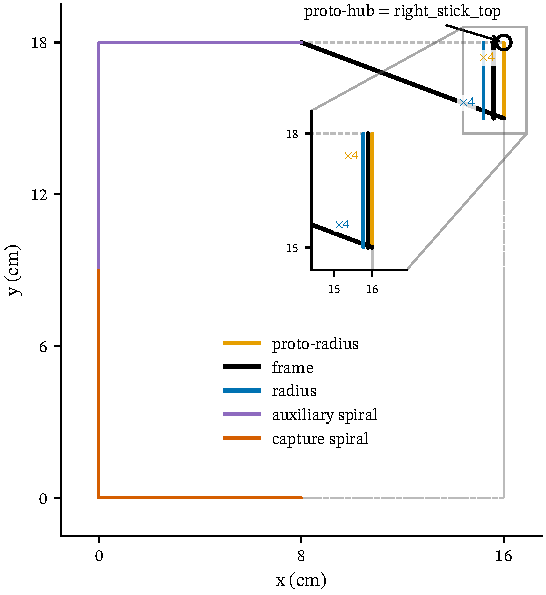
\includegraphics[width=0.7\linewidth]{figures/astar_fap/astar_web_final}
\caption{Final web of the committed A* plan (\code{visualization/\allowbreak{}plan\_data\_astar.js}, 26 actions,
75.5\,cm), replayed through the repository's primitive operators. Thread type is coloured as in all
other web figures; the dashed grey lines are the walkable supporting structure. The inset enlarges
the 3\,cm edge \code{right\_stick\_top}--\code{anchor\_right\_upper}, which carries four proto-radii,
four radii and one frame thread (parallel copies drawn slightly offset; $\times m$ marks
multiplicity). $n=1$ plan.}
\label{fig:astar_fap-web}
\end{figure}

\begin{figure}[htbp]
\centering
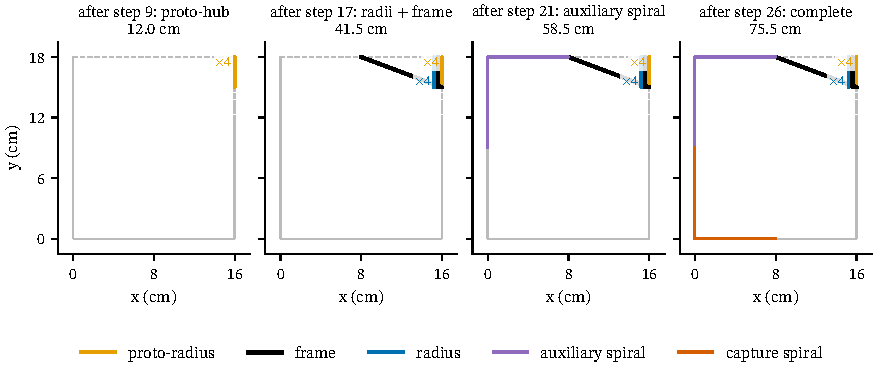
\includegraphics[width=\linewidth]{figures/astar_fap/astar_web_buildup}
\caption{Build-up of the committed A* plan: thread network after steps 9 (proto-hub marked), 17
(fourth radius and top frame thread), 21 (fourth auxiliary segment) and 26 (complete), with the
cumulative cost taken from \code{visualization/\allowbreak{}plan\_data\_astar.js}. $n=1$ plan.}
\label{fig:astar_fap-buildup}
\end{figure}

\begin{figure}[htbp]
\centering
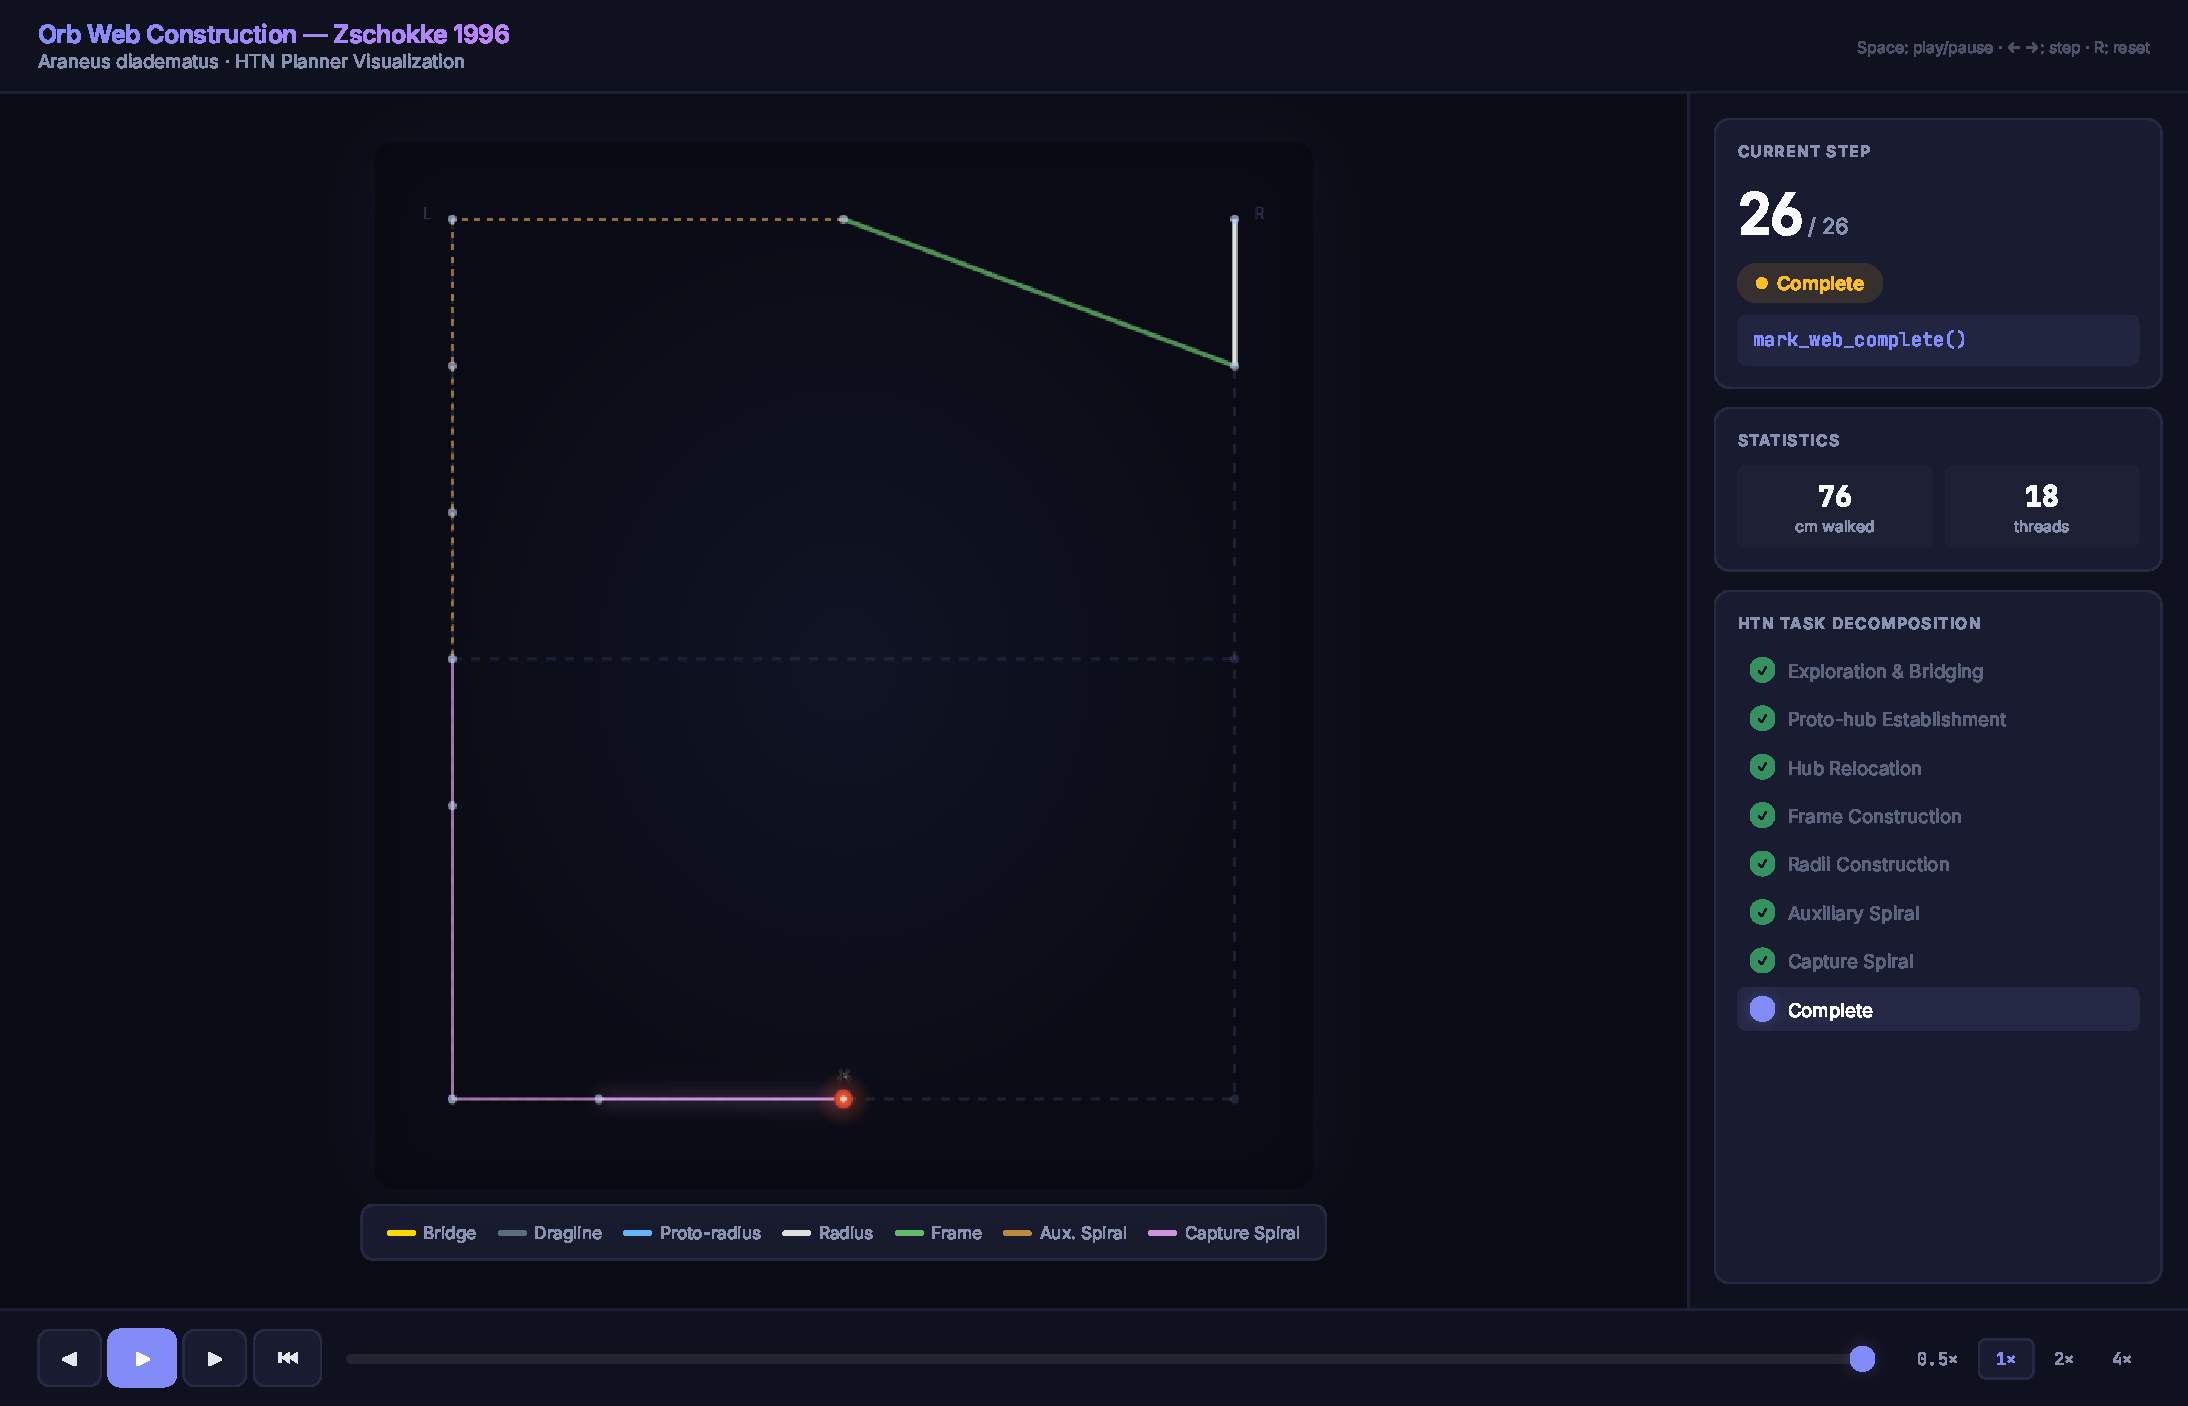
\includegraphics[width=\linewidth]{figures/astar_fap/ui_astar_final}
\caption{The repository's A* viewer (\code{visualization/\allowbreak{}index\_astar.html} with
\code{plan\_data\_astar.js}), captured in headless Chrome after jumping to the last step (26/26;
76\,cm walked, 18 threads). The page is a copy of the HTN viewer
(\code{spider\_web\_astar/\allowbreak{}make\_astar.py}), so its side panel still lists the HTN phases, including
``Hub Relocation'', none of which corresponds to an A* method. Unlike the current HTN viewer, the A* copy
cannot place \code{anchor@fraction} spiral nodes (irrelevant for this plan, which has none).
Capture script \code{scripts/\allowbreak{}astar\_fap/\allowbreak{}capture\_ui.sh}.}
\label{fig:astar_fap-ui}
\end{figure}

% --------------------------------------------------------------------------------------------
\subsection{The fixed-action-pattern model}
\label{sec:astar_fap-fap}

\paragraph{What ``fixed action pattern'' means in the code.}
\code{spider\_web\_fap} is a GTPyhop domain like the HTN models, but it encodes a different idea of
behaviour. Construction is five ``macro-stages'' (\code{run\_fap.py}): Y-shaped proto-web and frame,
radial spokes, auxiliary spiral, capture spiral with silk switch and recycling, and a
stabilimentum. Each is a compound task with exactly \emph{one} method (seven
\code{declare\_task\_methods} calls, one method each). Every method returns a fully ground
sequence whose only dependence on the state is a completion flag (and, for spokes, how many
spokes already exist). The top-level task is therefore a fixed concatenation
$\pi = \sigma_1\sigma_2\sigma_3\sigma_4\sigma_5\sigma_6$ of hard-coded subsequences. The planner
never chooses between methods, never binds a variable and never searches, so ``planning'' here
amounts to macro expansion. This is the main difference from the Checkpoint~2 HTN, whose
proto-hub task has three alternative methods. The FAP model has no opportunistic early phase, and
the whole construction is stereotyped. It also uses its own geometry (\code{FAP\_NODE\_COORDS}: a
16$\times$18\,cm frame with a hub at $(8,12)$, a stem anchor at $(8,0)$ and eight perimeter
points), starts the spider at \code{anchor\_top\_left} rather than \code{right\_stick\_top}, and
has its own operators (19 declared actions), including \code{switch\_silk\_chemistry},
\code{bite\_and\_recycle\_scaffolding} and \code{construct\_stabilimentum\_segment}.

\paragraph{What it produces.}
Our run (\code{61d18d8}) returns a 61-action plan costing 357.29\,cm. This equals both the
operators' own \code{energy\_expended} and the separate estimator in \code{main.py}. By stage:
Y-frame 5 actions, 54.0\,cm; spokes 24, 178.5\,cm; auxiliary spiral 10, 59.4\,cm; capture spiral 18,
59.4\,cm; stabilimentum 3, 6.0\,cm; finalisation 1. The final web (Fig.~\ref{fig:astar_fap-fap})
has three Y-frame threads, eight radii to eight distinct perimeter points, eight capture segments,
one auxiliary segment, three stabilimentum segments and the dragline of the initial drop. Seven of
the eight auxiliary segments are ``eaten'' during the capture spiral. The eighth survives because
the first capture segment (hub to \code{frame\_top\_left}) has no auxiliary segment to recycle.
The methods emit 72 primitive steps, but the plan has 61. GTPyhop~1.9.7 does not record an action
that leaves the state unchanged, so all eight \code{measure\_angle\_gap\_check} steps (the
``leg-calliper angle measurement'' of the spoke loop), the zero-length \code{walk(hub, hub)}, the
first non-matching recycle and the redundant \code{mark\_stabilimentum\_done} disappear from the
plan. The angle-measurement step is a stub that always succeeds, and the helper
\code{measure\_angular\_gap} is imported but never called. The spoke placement is hard-coded, so
no sensory feedback enters the model.

\paragraph{Behaviour when a precondition fails.}
Several operators check almost nothing (e.g.\ \code{climb\_up\_and\_out} only checks that the spider
is at the hub). Where a check does fail, there is no alternative. We perturbed the initial state in
three ways: spider released at \code{anchor\_top\_right}, spider released at the hub, and the stage-1
flag \code{y\_frame\_established} already set (stage~1 is then skipped and the first
\code{climb\_up\_and\_out} fails because the spider is not at the hub). In all three cases
\code{find\_plan} returns \code{False} in about 0.05\,ms. This happens under the installed default
strategy (iterative greedy, no backtracking) and under \code{iterative\_dfs\_backtracking} alike,
since with one method per task there is nothing to backtrack to.

\begin{figure}[htbp]
\centering
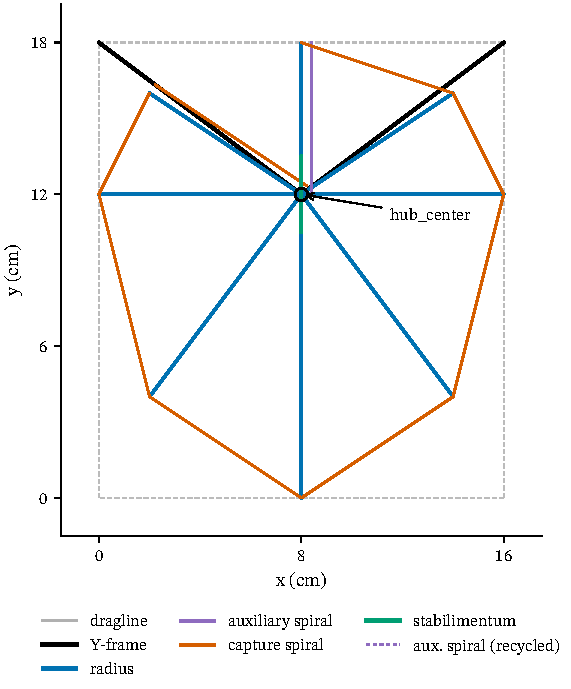
\includegraphics[width=0.7\linewidth]{figures/astar_fap/fap_web_final}
\caption{Final web of the FAP model (our run of \code{spider\_web\_fap} at \code{61d18d8}; 61 actions,
357.3\,cm). The Y-frame is drawn in the frame colour. Dashed purple: the seven auxiliary-spiral
segments laid and then removed by \code{bite\_and\_recycle\_scaffolding}. Dashed grey: the FAP
model's walkable perimeter, which differs from the Zschokke rig of the HTN and A* figures. $n=1$
deterministic plan; \code{runs.jsonl} tag \code{fap}.}
\label{fig:astar_fap-fap}
\end{figure}

% --------------------------------------------------------------------------------------------
\subsection{The ethological data table}
\label{sec:astar_fap-empirical}

\code{spider\_web\_astar/\allowbreak{}empirical\_data.md} (added with the A* package) tabulates values from
Zschokke~\cite{zschokke1996early} and secondary sources and maps them to four planned metrics
(success rate, efficiency ratio, adaptation time, decomposition depth). The values from Zschokke
include: 31 of 34 proto-radius constructions following one of six variants; 8 of 55 secondary frame
threads; 19 of 47 primary frames without a simultaneous radius; median exploration distance 5.61\,m
(simple structure, $n=37$ webs) and 27.60\,m (complex, $n=38$); median construction distance 13.64
and 14.37\,m ($p=0.096$). We spot-checked these against the PDF in the repository and found them
there. The table also lists Hesselberg and Vollrath's web geometry (capture area $239\pm16$\,cm$^2$
and others), marked \texttt{[CITED]}, not checked by us. It ends with a ``Predictions'' table
(for example ``A* nodes expanded grows $\gg$5$\times$'' with complexity) that no code tests.
\emph{No code in \code{spider\_web\_astar} reads this file.} Several of its numbers were later
copied by hand into the \code{empirical:} block of \code{spider\_web\_htn\_updated/\allowbreak{}config.yaml},
where the capture area (239\,cm$^2$) is the denominator of the efficiency ratio. The same medians
are quoted with the wrong unit in console output: both HTN \code{main.py} files print ``Zschokke
median exploration: 5.61\,cm'' where the source says metres.

% --------------------------------------------------------------------------------------------
\subsection{Side-by-side comparison on the Zschokke rig}
\label{sec:astar_fap-compare}

Table~\ref{tab:astar_fap-compare} and Figures~\ref{fig:astar_fap-webs}--\ref{fig:astar_fap-bars} put
the four planners next to each other. All four were run by us at the commits given. The HTN plans
are action-for-action identical to the committed viewer data (\code{plan\_data.js}: 128
actions, 751.6\,cm; \code{plan\_data\_updated.js}: 105 actions, 701.6\,cm). \textbf{These numbers
are not a like-for-like contest} (claim C17). The four planners differ in their goals, operators,
geometry and cost accounting:
\begin{itemize}
  \item \emph{Goal.} Both HTN plans build 4 frame threads, 8 radii to 8 anchors and full auxiliary
  and capture spirals (32 and 40 segments in the original HTN, 20 and 28 in the updated one). A*
  needs only 2 frame threads, 4 radii and 4+4 spiral segments, with no geometric condition. The FAP
  goal is ``all macro-stages done'' and includes a stabilimentum.
  \item \emph{Operators and cost.} The original HTN and A* share the same primitive operators and
  distance function. In the updated HTN (\code{config.yaml}) the spiral waypoints are generated as
  logarithmic and Archimedean spirals, which changes both thread count and length. The FAP model
  has its own operators. For example, \code{lay\_loose\_spoke} charges the outbound step and the
  return, and \code{tighten\_y\_frame} charges stem-to-hub.
  \item \emph{Geometry and start.} HTN and A* use the 17-node Zschokke rig with the spider released
  at the right stick top. FAP uses its own idealised frame and starts at the top left.
  \item \emph{Search.} The HTN and FAP plans come from GTPyhop's default iterative greedy
  decomposition. A* is a best-first search over a flat state space, with a heuristic that is
  either a constant per remaining item (\code{1e1bd44}) or zero (\code{61d18d8}).
\end{itemize}
Within those caveats the descriptive picture is this. The two HTN models build recognisable orb
webs with a hub, radii and interleaved spirals at 700--750\,cm. The FAP model builds a schematic
wheel at 357\,cm on a different frame. The A* plan is the cheapest (75.5\,cm) because it builds
almost nothing (Section~\ref{sec:astar_fap-web}). Planning times are milliseconds for the GTPyhop
models (FAP 2.4\,ms, original HTN 8.4\,ms, updated HTN 19.2\,ms; medians of 20 repetitions) and
0.58\,s for the committed A*. A* at the current commit returns nothing within its 120\,s budget.
The four runs do \emph{not} produce the same web, and the costs are not costs of the same task, so
they cannot be read as energy savings of one planner over another.

\begin{table}[htbp]
\centering
\small
\caption{Descriptive comparison of the four planners (not a joint quantitative conclusion; claim
C17). Times are the median (min--max) of 20 \code{find\_plan} calls in one process (HTN, FAP) or
of 10 processes with \code{PYTHONHASHSEED} 0--9 (A*), on one machine. A* plan cost: 75.54\,cm in
8 of 10 runs, 85.54\,cm in 2. Thread counts are of the final state. Source: \code{runs.jsonl},
\code{visualization/\allowbreak{}plan\_data\_astar.js}.}
\label{tab:astar_fap-compare}
\footnotesize
\setlength{\tabcolsep}{4pt}
\begin{tabularx}{\linewidth}{@{}>{\raggedright\arraybackslash}p{0.2\linewidth}*{4}{>{\raggedright\arraybackslash}X}@{}}
\toprule
 & Original HTN & Updated HTN & A* & FAP \\
\midrule
Package & \code{spider\_web\_\allowbreak{}htn} & \code{spider\_web\_\allowbreak{}htn\_\allowbreak{}updated} & \code{spider\_web\_\allowbreak{}astar} & \code{spider\_web\_\allowbreak{}fap} \\
Commit run & 61d18d8 & 61d18d8 & 1e1bd44 (61d18d8: no plan) & 61d18d8 \\
Planner & GTPyhop, greedy & GTPyhop, greedy & weighted A*, $w=3$ & GTPyhop, one method per task \\
Rig / start & Zschokke rig / right stick top & same (from \code{config.yaml}) & same as original HTN & own frame / top left \\
Plan length (actions) & 128 & 105 & 26 & 61 \\
Cost (cm) & 751.65 & 701.60 & 75.54 & 357.29 \\
Planning time (ms) & 8.38\newline(8.21--8.80) & 19.25\newline(18.55--20.31) & 576\newline(560--589) & 2.38\newline(2.31--2.57) \\
Frame / radii (distinct radius edges) & 4 / 8 (8) & 4 / 8 (8) & 2 / 4 (1) & 3 Y-frame / 8 (8) \\
Aux.\ / capture segments & 32 / 40 & 20 / 28 & 4 / 4 & 1 (+7 recycled) / 8 \\
Proto-radii / other & 4 / 2 bridge & 4 / 2 bridge & 4 / -- & -- / 3 stabilimentum, 1 dragline \\
\bottomrule
\end{tabularx}
\end{table}

\begin{figure}[htbp]
\centering
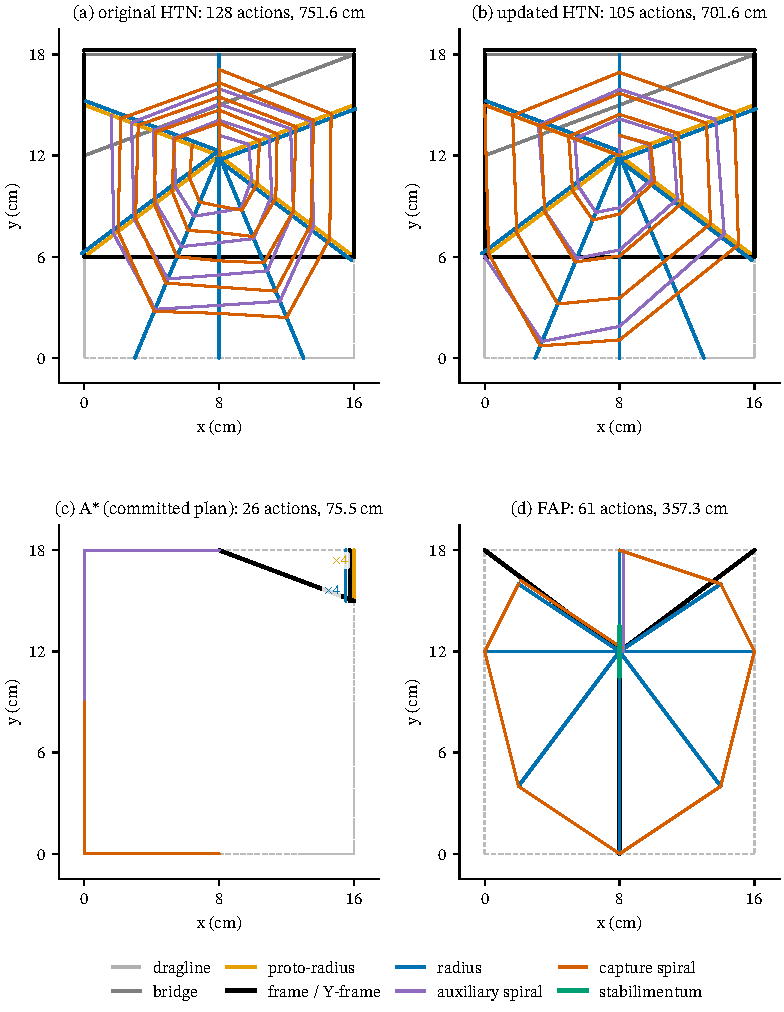
\includegraphics[width=0.9\linewidth]{figures/astar_fap/webs_four_planners}
\caption{Final webs of the four planners at the same scale (cm, equal aspect): (a) original HTN and
(b) updated HTN (our runs at \code{61d18d8}, identical to \code{visualization/\allowbreak{}plan\_data.js} and
\code{plan\_data\_updated.js}); (c) committed A* plan (\code{visualization/\allowbreak{}plan\_data\_astar.js});
(d) FAP (our run). Dashed grey: walkable supporting structure of each model, so (d) is drawn on the
FAP model's own frame. Thread colours as in all web figures; ``frame'' includes the FAP Y-frame.
$n=1$ plan per panel.}
\label{fig:astar_fap-webs}
\end{figure}

\begin{figure}[htbp]
\centering
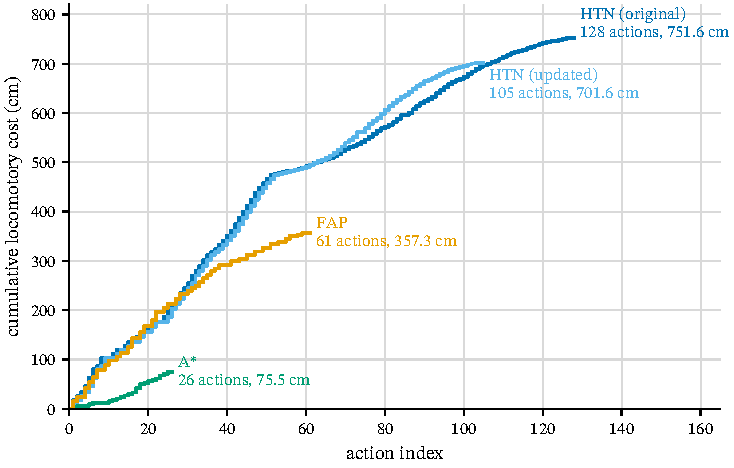
\includegraphics[width=0.8\linewidth]{figures/astar_fap/compare_cumcost}
\caption{Cumulative locomotory cost against action index for the four plans (HTN and updated HTN:
\code{cumulative\_energy} in \code{visualization/\allowbreak{}plan\_data.js} and \code{plan\_data\_updated.js};
A*: \code{visualization/\allowbreak{}plan\_data\_astar.js}; FAP: our run replayed through its operators). The
plans pursue different goals on different geometry (Table~\ref{tab:astar_fap-compare}), so the
curves describe each plan and do not compare efficiency. $n=1$ plan each.}
\label{fig:astar_fap-cumcost}
\end{figure}

\begin{figure}[htbp]
\centering
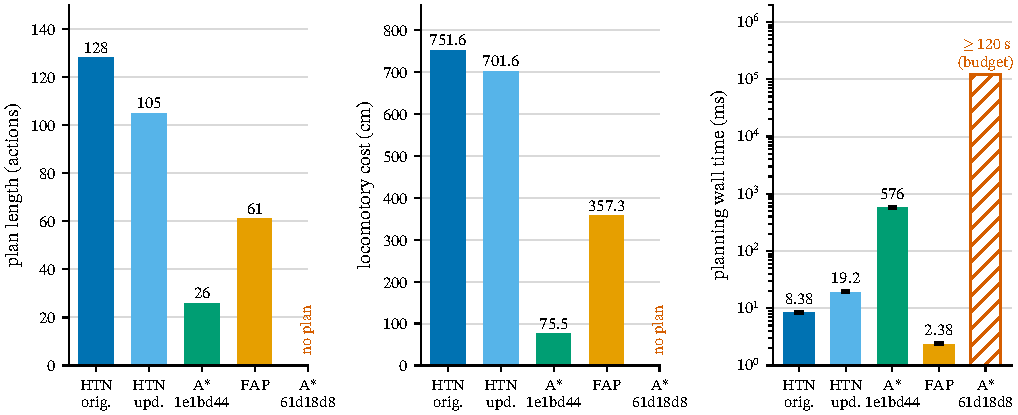
\includegraphics[width=\linewidth]{figures/astar_fap/compare_bars}
\caption{Plan length, plan cost and planning wall time for the four planners (and A* at the current
commit, which returns no plan within its 120\,s budget, hatched). Time bars: median; whiskers:
min--max over $n=20$ repetitions (HTN, updated HTN, FAP) or $n=10$ processes with different hash
seeds (A* \code{1e1bd44}). Log scale for time. The A* cost bar is the median (75.54\,cm; 2 of 10
runs gave 85.54\,cm). Source: \code{runs.jsonl}. Descriptive only (claim C17).}
\label{fig:astar_fap-bars}
\end{figure}

\paragraph{What this changes for the report.}
The Checkpoint~2 discussion argues that the HTN hierarchy reaches an efficient plan ``at a fraction
of the search cost that \ldots a flat-state search would require''. No flat-state search was
measured there. The only flat search in the repository is this A* planner. As committed it found a
plan in 0.58\,s, but for a much weaker and geometry-free goal. At the current commit it finds
nothing within 120\,s because its heuristic evaluates to zero. Neither result tests the claim,
which remains unmeasured. A fair test would need (i) the HTN's goal expressed as a state predicate
with geometric conditions, (ii) a working, and if optimality is claimed admissible, heuristic
(which requires handling the coincident nodes at $(8,0)$), (iii) a fixed hash seed or a
deterministic tie-breaker, and (iv) the same rig, operators and cost function as the HTN it is
compared with.
